%% ----------------------------------------------------------------
%% Thesis.tex -- MAIN FILE (the one that you compile with LaTeX)
%% ---------------------------------------------------------------- 

% Set up the document
\documentclass[a4paper, 11pt, oneside]{Thesis}  % Use the "Thesis" style, based on the ECS Thesis style by Steve Gunn
\newcommand{\setimp}{\newif \ifimp \imptrue}
\setimp

% Include any extra LaTeX packages required
\usepackage[square, numbers, comma, sort&compress]{natbib}  % Use the "Natbib" style for the references in the Bibliography
\usepackage[nottoc]{tocbibind} % bind bibliography to the table of contents
\usepackage{verbatim}  % Needed for the "comment" environment to make LaTeX comments
\usepackage{vector}  % Allows "\bvec{}" and "\buvec{}" for "blackboard" style bold vectors in maths
\usepackage[table]{xcolor}
\hypersetup{urlcolor=black, colorlinks=true}  % Colours hyperlinks in black, can be distracting if there are many links and colored blue.
\usepackage{graphicx}
\graphicspath{{Figures/}}  % Location of the graphics files (set up for graphics to be in PDF format)

%% ----------------------------------------------------------------
\begin{document}
\frontmatter      % Begin Roman style (i, ii, iii, iv...) page numbering

% Set up the Title Page
\title  {Your Thesis Title}
\authors  {Your Name}
            
\addresses  {\groupname\\\deptname\\\univname}  % Do not change this here, instead these must be set in the "Thesis.cls" file, please look through it instead
\date       {\today}
\subject    {}
\keywords   {}

\maketitle
%% ----------------------------------------------------------------

\setstretch{1.3}  % It is better to have smaller font and larger line spacing than the other way round

% Define the page headers using the FancyHdr package and set up for one-sided printing
\fancyhead{}  % Clears all page headers and footers
\rhead{\thepage}  % Sets the right side header to show the page number
\lhead{}  % Clears the left side page header

\pagestyle{fancy}  % Finally, use the "fancy" page style to implement the FancyHdr headers

%% ----------------------------------------------------------------
% Declaration Page required for the Thesis
\Declaration{

\addtocontents{toc}{\vspace{1em}}  % Add a gap in the Contents, for aesthetics

I, Myname , declare that this thesis titled, `THESIS TITLE' and the work presented in it are my own. I confirm that:

\begin{itemize} 
\item[\tiny{$\blacksquare$}] This work was done wholly or mainly while in candidature for an undergraduate degree at Cork Institute of Technology.
 
\item[\tiny{$\blacksquare$}] Where any part of this thesis has previously been submitted for a degree or any other qualification at Cork Institute of Technology or any other institution, this has been clearly stated.
 
\item[\tiny{$\blacksquare$}] Where I have consulted the published work of others, this is always clearly attributed.
 
\item[\tiny{$\blacksquare$}] Where I have quoted from the work of others, the source is always given. With the exception of such quotations, this project report is entirely my own work.
 
\item[\tiny{$\blacksquare$}] I have acknowledged all main sources of help.
 
\item[\tiny{$\blacksquare$}] Where the thesis is based on work done by myself jointly with others, I have made clear exactly what was done by others and what I have contributed myself.
\\
\end{itemize}
 
 
Signed:\\
\rule[1em]{25em}{0.5pt}  % This prints a line for the signature
 
Date:\\
\rule[1em]{25em}{0.5pt}  % This prints a line to write the date
}
\clearpage  % Declaration ended, now start a new page

%% ----------------------------------------------------------------

% The Abstract Page
\addtotoc{Abstract}  % Add the "Abstract" page entry to the Contents
\abstract{
\addtocontents{toc}{\vspace{1em}}  % Add a gap in the Contents, for aesthetics

The Thesis Abstract is written here (and kept just one page long or less). The page is kept centered vertically so can expand into the blank space above the title too\ldots Briefly, write in 3-4 paragraphs on what your project is about. This is a more precise version of your project abstract submitted on week 1 updated with developments between then and the submission time. Try to include the main features and functional requirements provided. As the title suggests this section is normally the only thing an executive would read so it MUST get across the main elements of the project.

}

\clearpage  % Abstract ended, start a new page
%% ----------------------------------------------------------------

\setstretch{1.3}  % Reset the line-spacing to 1.3 for body text (if it has changed)

% The Acknowledgements page, for thanking everyone
\acknowledgements{
\addtocontents{toc}{\vspace{1em}}  % Add a gap in the Contents, for aesthetics

The acknowledgements and the people to thank go here, don't forget to include your project supervisor (term one and two)\ldots

}
\clearpage  % End of the Acknowledgements
%% ----------------------------------------------------------------

\pagestyle{fancy}  %The page style headers have been "empty" all this time, now use the "fancy" headers as defined before to bring them back


%% ----------------------------------------------------------------
\lhead{\emph{Contents}}  % Set the left side page header to "Contents"
\tableofcontents  % Write out the Table of Contents

%% ----------------------------------------------------------------
\lhead{\emph{List of Figures}}  % Set the left side page header to "List if Figures"
\listoffigures  % Write out the List of Figures

%% ----------------------------------------------------------------
\lhead{\emph{List of Tables}}  % Set the left side page header to "List of Tables"
\listoftables  % Write out the List of Tables

%% ----------------------------------------------------------------
\setstretch{1.5}  % Set the line spacing to 1.5, this makes the following tables easier to read
\clearpage  % Start a new page
\lhead{\emph{Abbreviations}}  % Set the left side page header to "Abbreviations"
\listofsymbols{ll}  % Include a list of Abbreviations (a table of two columns)
{
% \textbf{Acronym} & \textbf{W}hat (it) \textbf{S}tands \textbf{F}or \\
\textbf{LAH} & \textbf{L}ist \textbf{A}bbreviations \textbf{H}ere \\

}

%% ----------------------------------------------------------------
% End of the pre-able, contents and lists of things
% Begin the Dedication page

\setstretch{1.3}  % Return the line spacing back to 1.3

\pagestyle{empty}  % Page style needs to be empty for this page
\dedicatory{For/Dedicated to/To my\ldots}

\addtocontents{toc}{\vspace{2em}}  % Add a gap in the Contents, for aesthetics

%% ----------------------------------------------------------------
\mainmatter	  % Begin normal, numeric (1,2,3...) page numbering
\pagestyle{fancy}  % Return the page headers back to the "fancy" style

\chapter{Introduction}
\label{chap:intro}
\lhead{\emph{Introduction}}
%This chapter should comprise around 1000 words and introduces your project. Here you are setting the scene, remember the reader may know nothing about your project at this stage (other than the abstract). N.B. The sections outlined in this document are suggested, some projects will have a greater or lesser emphasis on different sections or may change titles and some will have to add other sections to provide context or detail.
% Putting in comments within the TeX file can be really useful in making notes for yourself and dumping text that you intend to edit later

\section{Motivation}
My motivation for this project originated from my time on placement in McAfee. I was an intern Software developer on the Globalization Platform Development team. During my time I worked on numerous projects that are used throughout the company. 

Every so often our team would get emails from users saying they forgot their password, they can’t sign in or that an account needs to be created for them. These issues always went to a certain colleague and from speaking to him around the office I gathered it took way too long to solve these issues and that the process could be severely optimized.  Being such a busy company with a larger number of users these issues can waste valuable time which could be spent of more important problems. 

McAfee was also a fantastic place to work so I wanted to help out in any way I could, and this was a prime opportunity to do so.


\section{Contribution}
In this project I will be using many programming techniques. One important technique I will be implementing is the use of libraries and making my own libraries. This is a vital piece of the project as code needs to be reusable and interchangeable, when done correctly and as generic as possible libraries make this doable. 

 Another key programming technique is internationalization, the project being for a global company it must be useable in all languages. This can be achieved by not hard coding any strings, pictures, logos etc. All strings and such are kept in a single file and called when needed, the base English file can then be translated into another other language easily and cost effective.
 
This brings me to UI/UX design. I have complete control over this side of my project and user experience will be my main focus. I think it’s essential for users to get to their end goal in as little effort as possible while being aesthetically appealing. To do this I will be using HTML5 and CSS. 

Project management is another key aspect to this, being such a large project taking up so much time it needs to be managed correctly from the start. One way I will be managing my project is by having 3 different main git branches, production, QA and development. 

This brings me to the QA bit of the project as putting so much effort into something you would want a quality product at the end. Having these 3 branches makes this possible. When I think I’m done with a certain aspect of development I will be merging the development and QA branches. Then a QA team will be testing my project to ensure there are no defects and everything is working how it should be.

The leads me to early defect detection. This again is a vital bit to any project. A simple typo in your code could potentially break certain aspects and make them not work correctly which if not fixed could snowball and make the problem a lot worse than it needed to be. Using three different environments makes this possible as all a developer needs to do is tell the QA team what they have worked on and what it should do, and they will make sure of that. This lets the developer focus on developing and the QA team focus on finding defects. 

The final and probably most important part of my project is communication. Communicating with the client, gathering spec, updating the job status and just letting them know how everything is going. Communication is the most important bit to any project as functional requirements need to be clear and concise for both developer and client, so everyone can have a clear time frame on how long certain parts should take. 

\newpage
\section{Structure of This Document}
% notice how I cross referenced the chapters through using the \label tag --> LaTeX is VERY similar to HTML and other mark up languages so you should see nothing new here!
%This section is quite formulaic. Briefly describe the structure of this document, enumerating what does each chapter and section stands for. For instance in this work in Chapter \ref{chap:background} the guidance in structuring the literature review is given. Chapter \ref{chap:problem} describes the main requirements for the problem definition and so on ...
This document will be broken down into five chapters.

Chapter 1, as just read, introduces the project and defines the motivation behind doing it. It also breaks down the core software development technique's that will be used. 

Chapter 2, we will be reviewing what has been done before to get a better understanding of the approach we are going to take. We will also be looking at translation management systems in a whole to get an understanding of what our application will be working with. 

Chapter 3, defines the problem of current system while also stating the objectives that will be achieved upon project completion. The functional and non-function requirements are also stated in this chapter. This chapter is based around what must be done.

Chapter 4, is based around how the project will be achieved. Here we introduces the implementation approach to the project. It states the architecture and programming technologies that will be used. Defines the risk of the project. While also providing a schedule and finally a prototype.

Chapter 5, enumerates all the things that would be done if given more time and reflects on any problems encountered.  % Introduction
\chapter{Background}
\label{chap:background}
\lhead{\emph{Background}}
The key question to answer in this chapter is: "What has been done/is being done". 

This chapter comprises around 4000 words and should put your project into context within Computer Science. Your focus here should be on the final section "Current State of the Art". This should be at least 2500 of the 4000 words of this section.

\section{Thematic Area within Computer Science}
Position your topic within Computer Science. This activity will aid you in your literature review also. We zoom out to see three levels:

% notice the enumerate structure to create itemized lists
\begin{enumerate}
    \item What is the core topic your project is about? e.g., Mobile app for online voting.
    \item What core area(s) does the project fall under? e.g., Mobile applications, Social Networking, Service Providers. 
    \item What main area(s) of Computer Science does the project fall under? e.g. Software Development, Cloud Computing.
\end{enumerate}

The ACM Computing Classification System (http://www.acm.org/about/class) will aid you in this, use the 2012 categories. Make sure to use figures and illustrations were appropriate. LaTeX will take care of the formatting of these. Do not try to get fancy here, you should concentrate on the content and not the formatting, this is why we are specifying LaTeX.

% Again take note of the structure, simply copy and paste this for future single figures
\begin{figure}[ht]
  \centering
      \includegraphics[width=0.7\textwidth]{successkid.jpg}
  \caption[A picture of the success kid!]{A picture of the success kid!\cite{Reference1}}
  \label{fig:successkid}
\end{figure}

You can specify the width and label for a figure which allows you to reference the figure and you can attribute a source in the figure caption as is done for figure \ref{fig:successkid}. Make sure you reference all external figures (i.e. figures you did not create yourself). Also use references for all figures e.g. use "... in figure \ref{fig:successkid} ..." NOT "... in the figure above ...".

\section{A Review of -INSERT THEMATIC AREA-}
The focus of this section is at the heart of the project research phase. You must identify the main sources of information you should be aware of within your chosen area and pay regular attention to so as to strengthen your knowledge in the core topic you are working at. So here you should develop an knowledge of not only your core topic but also about the area of computer science the topic falls under. More specifically you should research the following:
\begin{itemize}
    \item The top 5 International Conferences and Journals most related to your topic. This is crucial, as it represents the main source for keeping you aware of what the state-of-the-art in your topic is.
    \begin{itemize}
        \item In particular it will make you aware of what other projects related to yours have been already done (so that you can compare/position your project w.r.t. these).
        \item What new techniques are being developed, so that you can apply them in your work. e.g. new frameworks for data visualization
    \end{itemize}
    \item The top 3 most recent books/texts related to your topic. There are many free resources from which you may download a relevant text on the topic of your project. Try to either download or borrow 3 recent (no older than 10 years) texts relating to the topic your project is on which you will use throughout the project as reference material and to aid in tackling a number of the technical problems you may encounter. Any PhD/MSc thesis that have published in the last 5 years relating to the topic are also invaluable resources as they will contain a state of the art and references in your project topic. Approach these only after reading/viewing the wikis/Youtube videos you find as a certain level of knowledge will be assumed about the topic.
    \item The top 5 companies/organizations potentially interested in the product you are developing. Finally, this is also crucial, as it forces you extend to purely programmer view of the project to a wider view considering the market, potential stakeholders and niches where your product can become useful. Moreover, Computer Science is a huge topic with loads of different works and roles. If you pick a project in the area you feel passionate about, and you identify what the market in this area is about, then you can drive your future professional career (from the very beginning) towards the path that makes you happier. I know that this does sound as a very technical reason, but I suppose we all agree is probably the most important of all reasons for choosing a particular project focus. 
    \item The top 5 wiki/forums/blogs/Youtube channels most related to your topic. This is crucial to you as well, as it represents a more accessible, personal and less informal way of communication with people working/interested on the same topic as you are. This communication is extremely helpful for improving your skills, solving potential doubts and increase the interest/relevance of the topic/area itself.
\end{itemize}

You should begin your journey of discovery in reverse order to the listing above (which is given in order of academic importance/significance). So when you are researching your topic first look up some TedX talks or youtube tutorials, then research what companies are doing in the area, then get a handful of very good texts on the core topics of your area (anything older than 5 years usually is not helpful here) and finally start reading conference or journal papers (again newer is better here). In particular during this section you may need to use tables to list resources. These are also automatically formatted in latex thus allowing you to concentrate on content. for example table \ref{tab:Mylar}.

\begin{table}[ht]
	\centering
		\begin{tabular}{ c  c  }
		\hline
		\hline
		Parameter & PET \\
		\hline
		Youngs Modulus & 2800-3100MPa \\
		Tensile Strength & 55-75MPa \\
		Glass Temperature & 75$^\circ$C \\
		Density & 1400kg/m$^3$ \\
		Thermal Conductivity & 0.15-0.24Wm$^{-1}$K$^{-1}$ \\
		Linear Expansion Coefficient & $7\times10^-5$ \\
		Relative Dielectric Constant @ 1MHz & 3\\
		Dielectric Breakdown Strength & 17kVmm$^{-1}$\\
		\end{tabular}
	\caption{PET Physical Properties}
	\label{tab:Mylar}
\end{table}

What has been done before in your community w.r.t. your topic? Once you have gotten an understanding of the topic and technologies and have identified the top 5 formal conferences/journals, wiki/forums/blogs/Youtube channels and companies/organizations the next step is to research in depth on them! And here in depth means in depth. Make sure you cite\cite{Reference1} a number of papers \cite{Reference3}, luckily Latex will take care of the ordering of the citations \cite{Reference2} for you.

The aim here is that you find the trends in your topic (3), and more in general in the area in which your topic resides (2) your project falls under and from these trends you develop your initial project question further and begin to get insights into how others have solved/approached similar problems. Think of this section as colouring in your initial idea. Before you approach this section you should read at least 4/5 good literature reviews (a selection of last years projects will be posted on blackboard to aid you but you should find other sources also).

In particular in this section, you must find and analyze at least 5 (ideally around 10) works belonging to, or at least related to, your work. You must describe these works and position your project w.r.t. them (i.e., clearly identify the similarities and differences between your project and each of these works). Also remember if you find that you are detailing topics that you have not introduced already here you need to add something to the earlier Scope section. % Background Theory 
\chapter{Problem - GlobalSight User Management System}
\label{chap:problem}
\lhead{\emph{Problem Statement}}

\section{Problem Definition}
GlobalSight is a Globalization Management System. It contains a translation management system, and a complimentary work-flow management system. It’s the primary tool for getting McAfee productions, documentation, and websites translated. McAfee translate into over 60 languages, and variants. GlobalSight is also used as a LDAP substitute for other internal systems, where integration with Active Directory is not possible, or desired.

Multiple servers are used to share load, and to ensure segregation of business content streams. McAfee also have separate development and staging/UAT environments. There are currently twelve separate servers in use. Production server, at least, of each content stream is externally facing, and is accessed by translators worldwide, to complete their translation work.

At present, more than 1500 unique active users on the system, between translators and internal users. Each user is on each of the 12+ servers. When a user is created, or their password
updated, that change needs to be replicated to each server.

It currently takes about 25 minutes to change 1 password, and about 30 minutes to create a single use on all systems.


\section{Objectives}
To create a web portal application that will allow easy management of user in the GlobalSight environment.  GlobalSight has a published API set, which includes API’s to manage users, which should be used by the application.

The application should have the ability to adjust dynamically as more servers are added to the cluster, and where some are removed/decommissioned. 

The application will be safe from a security point of view, having so many users data protection is key. Mcafees' own security team will be running regular checks for vulnerabilities in the system.

\section{Functional Requirements}
The application will have the ability to differentiate between a normal user and an administrators. Administrators should have the ability to which users can log in to the system and disable a user's log in if required. Administrators will also have the ability to manage the server list.

The application be able to define server groups, so users can group the production, development and UAT servers of a content stream together. A server can only exist in one group. This includes the main server, it’s details are not stored in the database, but it’s assignable to a group. A server must be part of a group, but a group can contain one server. There’s no limit to the number of servers in a group. A group can have zero members, and not show in the UI for app users, but still exist. It should be possible to delete or make inactive a group. Deleting a group removes it from the database, while machining active just removes sets an “inactive” flag in the database. There’s no need for a UI to show inactive servers, not is there a need for functionality to make them active again. That can be done via database directly. A group cannot be deleted or made inactive, if it still has members. 

\pagebreak


\section{Non-Functional Requirements}
The UI for will be minimalistic, allowing for users to easily traverse the application in the most efficient way.  
All content such as strings, images and colours will be externalized to separate files to allow for the application to be fully translated in future. 

The application will be reliable, users cannot access their accounts and the application is down for some reason that could potentially leave workers with no ability to actually achieve their work.




 % Problem
\chapter{Implementation Approach}
\label{chap:implementation}
\lhead{\emph{Implementation Approach}}

\section{Architecture} \label{sec:Arch}
This application will have a HTML5, CSS3 and AngularJS front-end. Here is where the general look of our application will be done.
\begin{itemize}
    \item HTML5 provides the structure of the web application. Tags are used to describe the visual representation of the application, these are the building blocks of web pages. Tags are not displayed but they are used to render the content to the page. 
    \item CSS works in conjunction with HTML. It describes how the HTML elements are to be displayed on screen. This is particularly useful for viewing the application no different screen sizes. CSS allows for a dynamic and responsive web page. 
    \item AngularJS is a structural framework for dynamic web apps. It allows use of HTML as a template and enables the extension of HTML's syntax to express the application's components in a brief and clearly expressed manner.
\end{itemize}
This work will be done using Sublime Text 3 as this has lots of useful shortcuts that will reduce development time. 

The logic of the application will be done using a C Sharp back-end. Here is where our checks and general operations will be written. C Sharp is one of the most popular programming languages out there as it has many uses so this will come in useful when debugging and general fixes as there is a lot of documentation and helpful information out there. It's also useful for maintaining code as easily readable for programmers. This work will be done using Microsoft Visual Studio. 

The database chosen for this is Microsoft SQL Database. This being another Microsoft product, visual studio provides native support for programming with Microsoft SQL Database. Microsoft SQL Database can be used to visually observe and analyze queries and optimize the database performance. Tables can also be easily maintained and altered adding or removing columns where necessary. An important point to make about our database too is that passwords will not be stored, encryption will make this possible.

Unit and end too end tests will also be used to maintain code. These are often overlooked in projects but are absolutely vital. The logic will be tested by our unit tests, here we test that a function works as intended, end too end tests then test the UI of our application. Here we test things such as a button bringing you to the correct location. These tests are so important for large projects because when implementing new functionality it could unexpectedly impact old functions. These tests will be run using Jenkins continuous integration tool. This way we can automate the testing of our code and be notified of any defects immediately.

All source code will them be stored in internal GIT repositories. These repositories make having different environments possible, such as the development, QA and production environments. 

The application will be managed through JIRA. JIRA is an issue management platform that allows easy management of issues throughout their entire lifecycle. It is highly customizable, and can be tailored to fit any workflow. It will be used to manage and track development, and is useful for sticking to time frames. 

\section{Risk Assessment}
The application will be regularly tested by McAfees security team for threats so by the end of the project any security flaws should be mitigated. User data is the heart of the application and if not attended too properly could lead to some fatal problems. Having 1500+ users, all of whoms data will be on 12+ servers protecting their information and keeping it consistent is vital. Not keeping data consistent could lead to some users not being able to use any internal McAfee applications. To sign into an applications users passwords must be the same on all servers. This could lead to a potentially disastrous scenario. For instance imagine we go to change a users password and we manage to do it on 11 servers but the final one is down and we miss this server, now we have inconsistent data which cannot happen. This scenario will have to be handled with care, before doing any operations we will have to check the servers and their availability. That's one way to deal with this potentially catastrophic error but what happens if we check the server availability and they're all good but as we traverse through one goes down, well then we have the same problem. To deal with this scenario we will have to implement a three-way handshake when changing users data along with a revert option if all servers don't respond.  

\section{Methodology}
For the development of this application an agile approach will be taken. This is where the different development environments come in useful. Development can be done in the development environment while testing can be done in the QA environment simultaneously. These different environments allow the ability to easily change things as we progress. Requirements are realistically always going to change throughout a project and that's why the agile methodology is the best one to follow. 

The use of JIRA is also vital for this methodology. The QA team can report any defects or bugs they find and create a job on JIRA. The QA team can then see that their issues are being worked on and for how long. This is where spring planning comes into the frame. Here the product owner and development team go through the application backlog and prioritize issues, while also providing acceptance criteria for completion. This is a skill that is often overlooked in Computer Science, communication is key to absolutely everything so developers and product owners need to be able to converse so that the product owner knows what's being done and so the developer knows what is to be done. 


\section{Implementation Plan Schedule}
The development process will start in early January. This will include setting the project up on GitHub along with all the different environments it needs. During this time, heavy emphasis will be put on the structure of the project, this is very important as a good foundation is vital as it will make it easier to update and maintain in the long run. 

Come February the plan is to have general functionality working and for the development environment to be live. The point of having this environment is to test what has been implemented so far and get a feel for application and get a better understanding of how the application will work in the real world. 

By the middle of March our QA environment should be live. Here the McAfee quality assessment team will be testing the application for any bugs while also giving suggestions on changes this could range from something as simple visual changes or a complete flow change. 

April will be bug fixing and any minor tweaks that need to be done. Here we should be on the final stage of the project so it's all about fine tuning.

May the production environment will be live. This will be a fully functional application that will be getting real world use by many users. Therefore the QA and bug fixing stage is vital as the QA team may see problems where a developer may not.

\begin{figure}[ht]
  \centering
      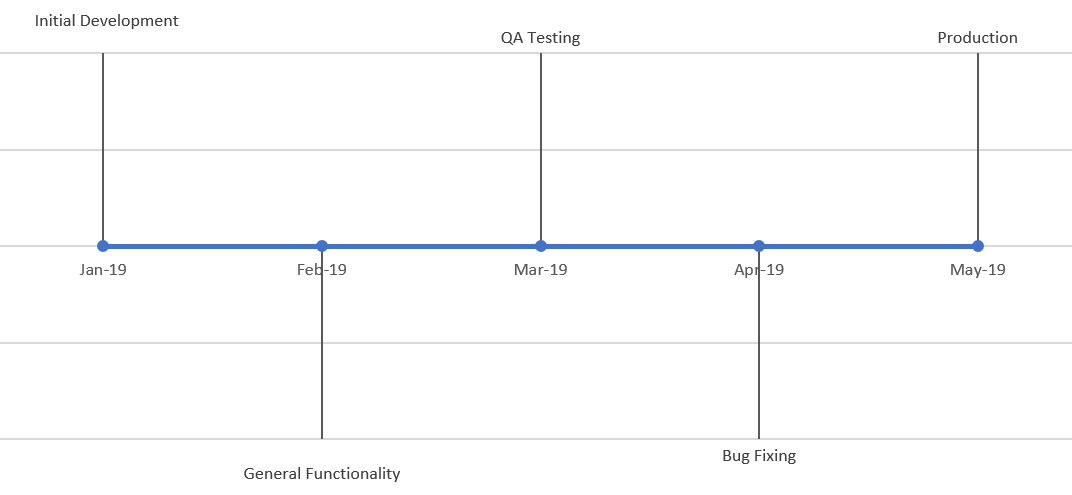
\includegraphics[width=1\textwidth]{MilestoneDiagram}
  \caption[Milestone Diagram]{Milestone Diagram}
  \label{fig:milestoneD}
\end{figure}

\section{Evaluation}
The number of bugs the project has will my main focus for the evaluation. If a project has even a lot of bugs, whether they are minor or major they make an application feel sloppy and unprofessional. Even something as simple as spelling mistakes or buttons getting misaligned when translating the application to another language can give a user a bad impression which could lead to loosing users.

Threat detection is another major part of the evaluation. This project will have thousands of users across multiple servers and their data must be kept secure. McAfees security team will be running regular checks on the application to make sure it is safe for all users. Threats can come from many areas of a projects, a simple one would be not checking input from a text box. All data entered by a user should be put through a black list check. The black list would contain things such as backslashes and double dots, these can be used by hackers to traverse the applications files and folders and potentially even run a cmd where anything would be possible from there. That's why threat detection and prevention is a vital focus.

The speed and responsiveness of the application is also another factor we must take into consideration. The applications code must be optimized to it's fullest. A sluggish application is unprofessional and cannot happen when it's being used for a business. The size of the project needs to be kept as low as possible as this will have a major impact on the load time, this can be done by making sure code is not duplicated or something as simple as making sure there are no unnecessary empty lines as these can increase file size. 

Readability of code is another important aspect to the project. This application will be used for potentially years and will be maintained and updated by numerous developers. Code should be easy to understand and well commented. 

\section{Prototype}
As stated previously a basic simplistic approach to the look of this project will be taken. This is necessary to give a intuitive nature to the application. our admin will be greeted to something like so. 
\begin{figure}[ht]
  \centering
      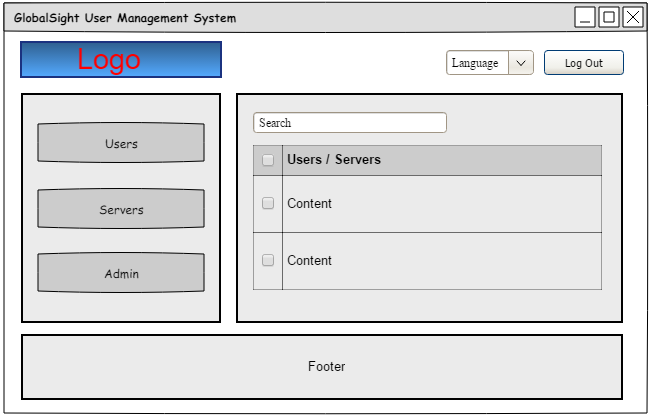
\includegraphics[width=1\textwidth]{Prototype1}
  \caption[Prototype 1]{Prototype 1}
  \label{fig:proto1}
\end{figure}

Our admin will be able to view our users and servers right away. Both will have the same table look with just different content. Our admin can then click on the desired user/Server where they can do their desired task such as reset password, set server groups etc. 

Upon clicking on an element such as a server our users will be greeted with a view like this. 
\begin{figure}[ht]
  \centering
      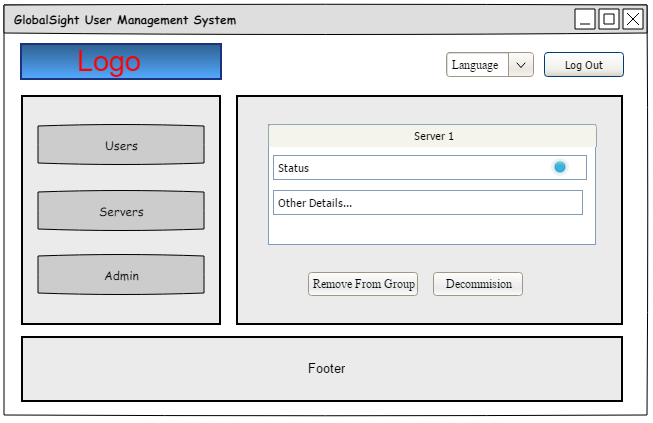
\includegraphics[width=1\textwidth]{Prototype2}
  \caption[Prototype 2]{Prototype 2}
  \label{fig:proto2}
\end{figure}

As you can see we plan on keeping the application looking more or less the same when traversing it again to give that intuitive feel.  % Solution Approach

\ifimp
\chapter{Conclusions and Future Work}
\label{chap:conclusions}
\lhead{\emph{Conclusions}}

\section{Discussion}
The main problem I encountered during this is chapter two the research phase. Being given a project from McAfee a lot of the background information was already done and a lot of my research was talking to the development team and information gathering from the managers. Going forward having this style of interaction will be helpful as this is different to a lot of students but it was hard to put into words what was done. Communication is a big part of any project so I am grateful for this experience. 

Another problem is not having information on the data that will be going into our database. This just made it virtually impossible to plan our database in advance but once we're hands on working in McAfee this will become clear. 

\section{Conclusion}
Our problem is a simplistic one in a sense, many users that are being mishandled leading to a waste of time and resources. The solution is also simplistic to define. Centralize all users to a single application where an admin can control them and give support. Such a simplistic problem definition and solution has a rather complex implementation. The sheer amount of users and servers could lead to many problems. Servers could go down which our application will have no control over, our application speaking to other applications will be difficult and there is a lot of sensitive user data that has to be handled with care. Putting a lot of thought into our agile methodology is the pivotal point to make this project work. Having different environments for development, QA and production is what will make this work. 

\section{Future Work}
Given more time I would have implemented more diagrams to convey points better. Textual information is a good base to have but visual information helps wrap your head around things, while adding a nice aspect to the whole document.  % Conclusions and Term 2 work
\chapter{Testing and Evaluation}
\label{chap:eval}
\lhead{\emph{Project Testing}}
The goal of this chapter is an objective evaluation of the final system. The evaluation must be quantitative and not qualitative. You may perform qualitative evaluation but this should not form the basis of the main conclusions you derive from the evaluation. This evaluation, where possible, should be comparative, i.e. you should evaluate your system against a commercially available system and/or system detailed in a research publication. You should demonstrate operational testing of the project using real or contrived data sets to evaluate aspects of the project not encompassed in the software testing (e.g. quantify how well does your project achieved the overall goal). 
\begin{itemize}
    \item For software based projects this will include, but should not be limited to, evaluation of non-functional requirements.
    \item For infrastructural projects this testing should include system/network KPI analysis.
    \item For analysis based projects (ML, malware or other) this may include model evaluation or YARA rule validation, for example.
    \item For management projects, where software testing or infrastructure testing may not be in scope, the test process for the system is expected to be more rigorous and well described than a project incorporating significant development work.
\end{itemize} 

Some suggested sections (the nature of this chapter should be discussed in detail with your term 2 supervisor):

\section{Metrics}
Identify and describe the metrics you used to evaluate your project. You should have identified some of these in the research phase report but will detail these as you progress through the design.

\section{System Testing}
Describe the experimental setup for each metric, and how you obtained the measurements. Describe the inputs for each experiment

\section{Results}
Summarise the output data, and the statistical or other techniques to deduce your results. Summarise your results, including tables or graphs as appropriate with a brief description of each. here possible, compare your results with other products/systems. Identify any possible threats to the validity of your results, and discuss each briefly here (you will discuss in more detail in the next chapter). % Conclusions and Term 2 work
\chapter{Discussion and Conclusions}
\label{chap:conclusions}
\lhead{\emph{Discussion and Conclusions}}
In this chapter, you should expand upon (and initially reflect upon) the discussion and conclusion of the research phase of the project. The expectation here is that you should discuss the results presented in the previous evaluation section of the project in their totality (i.e. as a whole) from which you will then draw clear conclusions both on the quantitative and qualitative aspects of the overall project. This chapter should be a about 2000 words long (5 pages of text - 1600 words of discussion and 400 words of conclusion). This may vary depending on quality. The conclusion section of this report should conclude the project.

Some suggested sections (the nature of this chapter should be discussed in detail with your term 2 supervisor):

\section{Solution Review}
Discuss how well your solution solves the problem, based on your results from the evaluation chapter.

\section{Project Review}
Discuss how well you addressed the project, and what you might do differently if you were to do it again. Make sure to identify how you handled any problems that arose during the project. Identify key skills that you learnt during the project, and clearly describe how you applied these, and how you might apply them differently if you were to do a similar project.

\section{Conclusion}
Enumerate the main conclusions you have got in terms of background, problem description and the solution approach you have come up with. Detail your primary and any secondary conclusions from your project.

\section{Future Work}
Discuss any proposals for completion of the project, or for enhancements, or for re-design of your solution or software. Enumerate all the things you would have wanted to do should you have more time to work on this project. % Conclusions and Term 2 work
\else
\chapter{Conclusions and Future Work}
\label{chap:conclusions}
\lhead{\emph{Conclusions}}
This chapter should comprise 2-3 pages and enumerate conclusions of this phase of work. In your final report Discussions and Conclusions will form separate chapters and be significantly longer and more detailed.

\section{Discussion}
A reflective discussion of some of the problems you encountered during this phase of the project and how that may influence how you proceed with the next phase.

\section{Conclusion}
Enumerate the main conclusions you have got in terms of background, problem description and the solution approach you have come up with.

\section{Future Work}
Enumerate all the things you would have wanted to do should you have more time to work on this report.

Additional resources on the use of latex is below.

Tutorials:
\begin{itemize}
    \item \url{https://www.latex-tutorial.com/tutorials/beginners/how-to-use-latex}
    \item \url{https://en.wikibooks.org/wiki/LaTeX}
    \item \url{https://www.sharelatex.com/learn/Main_Page}
    \item \url{http://www.math.harvard.edu/texman}
    \item \url{https://web.stevens.edu/hfslwiki/images/a/a0/ShareLatex_Tutorial.pdf}
\end{itemize}

Presentations:
\begin{itemize}
    \item \url{http://www.iu.hio.no/~frodes/rm/ppt/latex.ppt}
    \item \url{https://classes.soe.ucsc.edu/ams200/Fall09/Latex_intro.ppt}
    \item \url{http://www.menet.umn.edu/~blake/latexcourse/courseslides.ppt}
\end{itemize}
 % Conclusions and Term 2 work
\fi
%% ----------------------------------------------------------------
\label{Bibliography}
\bibliographystyle{IEEEtranN}  % Use the "IEEE Transaction" BibTeX style for formatting the Bibliography
\bibliography{Bibliography}  % The references (bibliography) information are stored in the file named "Bibliography.bib"
\lhead{\emph{Bibliography}}  % Change the left side page header to "Bibliography"

%% ----------------------------------------------------------------
% Now begin the Appendices, including them as separate files

\addtocontents{toc}{\vspace{2em}} % Add a gap in the Contents, for aesthetics

\appendix % Cue to tell LaTeX that the following 'chapters' are Appendices

\input{Appendices/AppendixA}	% Appendix Title

\input{Appendices/AppendixB} % Appendix Title

%\input{Appendices/AppendixC} % Appendix Title

\addtocontents{toc}{\vspace{2em}}  % Add a gap in the Contents, for aesthetics
\backmatter
\end{document}  % The End
%% ----------------------------------------------------------------